\subsection{Results}
\label{sec:results}
The design \& implementation of cloud analytics plaform was described
in sections \ref{sec:design} and \ref{sec:implementation}. The final
deliverables are two images named db-deliverable and dev-deliverable
which are stored in the GPFS under the team1 directory. In the rest of 
this section we discuss how this analytics platform can be used by the
user for data analytics.

We followed a simple use case of gathering all currency related data
from NCSU website and bringing all gathered data into structured form.
The above mentioned use case contains four important steps:
\begin{enumerate}
  \item \textbf{Gather the data}: First of all, to do any kind of data analysis
    some data needs to be collected. Here it was necessary to gather
    all data from NCSU website. When it comes to gathering lots of
    data from the internet, using an automated tool like Nutch is
    always a good approach. Our platform was designed to make Nutch
    available to the platform user. For our use case Nutch was configured
    to crawl all web pages present on NCSU website and gather all
    information present on these web pages. The data gathered by Nutch
    was stored into Apache Solr for further processing.
  \item \textbf{Filter the data}: The amount of data gathered by Nutch was
    huge. The requirement was to only keep relevant pieces of information
    from the gathered data. Filtering the data without losing relevant
    content is a difficult task. To achieve this we used Mortar
    toolkit. Mortar provides a technique of mind map for filtering the relevant
    data. Mortar processed the gathered data present in Solr, filtered
    it and stored the filtered data back into Solr.
  \item \textbf{Annotate the data}: The filtered data was now present in
    Solr. However, this data could not be queried using specific
    keywords. To allow this kind of queries on filtered data it was
    necessary to add certain metadata or annotations to the filtered data.
    The filtered data was annotated using Apache UIMA annotator
    functionality. An annotator jar was created and injected into Solr to annotate
    filtered data.
  \item \textbf{Represent the data}: Accessing the annotated data stored in
    Solr was still not convenient because the data was not present in
    a structured form. To represent the data in structured format it was exported
    into PostGres relational database. Further, Portrait was used to
    visualize the structured data stored in PostGres. This data was
    then queried to get specific information about a particular currency.
\end{enumerate}

The data crawled by Nutch was around 450 KB in size and contained 46
documents (Figure \ref{result-nutch-core}). After
filtering the data using Mortar, size was reduced to 320 KB and it
contained only 36 documents (since Mortar keeps only relevant pieces
of information). This can be seen in Figure \ref{result-mortar-core}. 
Finally the data was annotated (Figure \ref{result-uima-core}) and
exported into PostGres. Data visualization using Portrait can be seen
in Figure \ref{result-portrait}. 

\begin{figure}
  \centering
  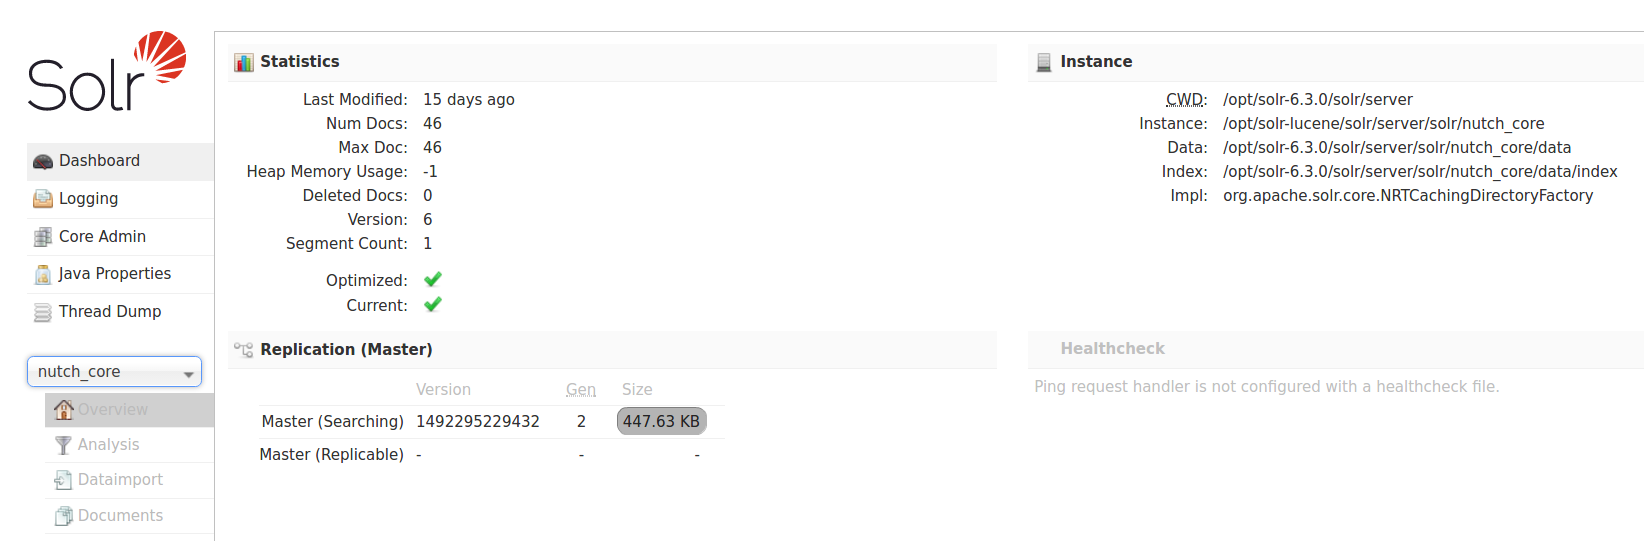
\includegraphics[width=15cm,height=6cm]{screenshots/result-nutch-core.png}
  \caption{Data crawled by Nutch - Indexed by Solr}
  \label{result-nutch-core}
\end{figure}

\begin{figure}
  \centering
  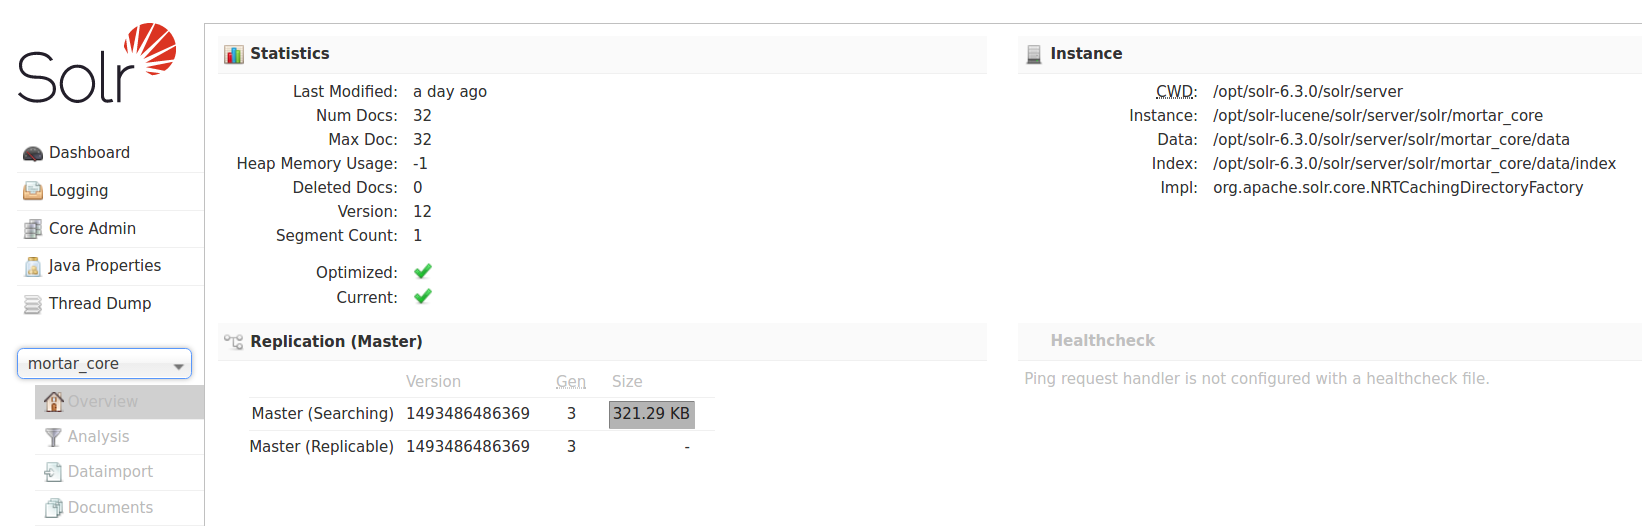
\includegraphics[width=15cm,height=6cm]{screenshots/result-mortar-core.png}
  \caption{Data filtered by Mortar - Indexed by Solr}
  \label{result-mortar-core}
\end{figure}

\begin{figure}
  \centering
  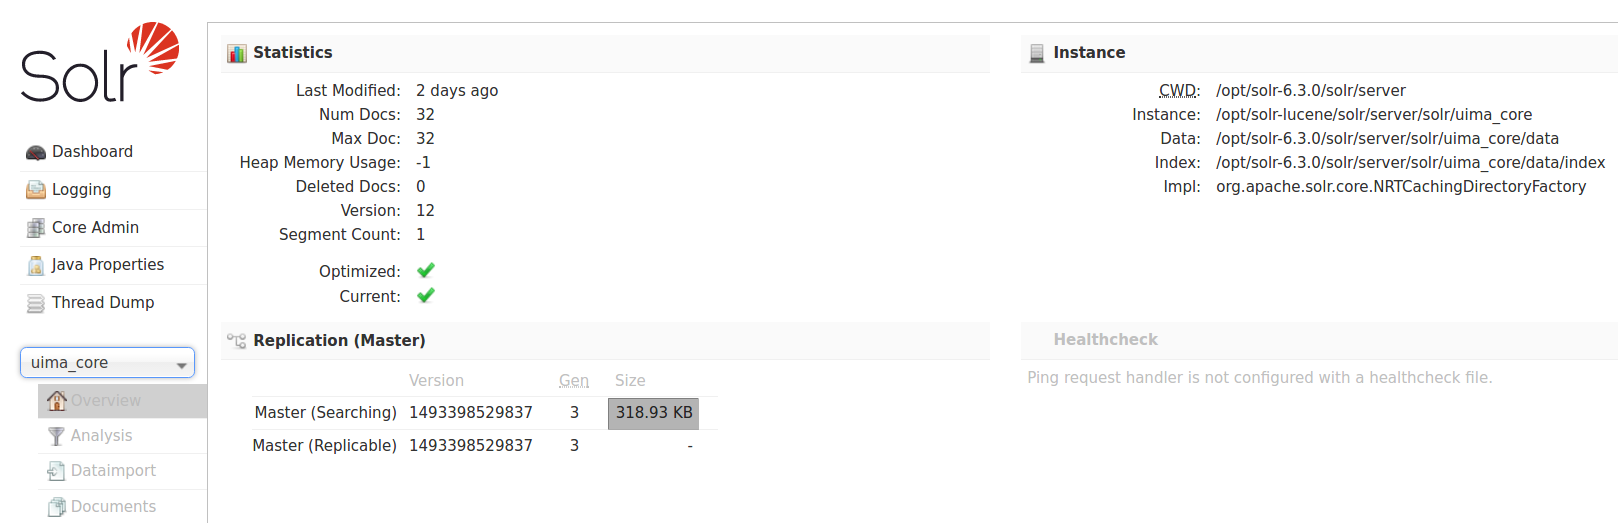
\includegraphics[width=15cm,height=6cm]{screenshots/result-uima-core.png}
  \caption{Data annotated using Apache UIMA}
  \label{result-uima-core}
\end{figure}

\begin{figure}
%%  \centering
  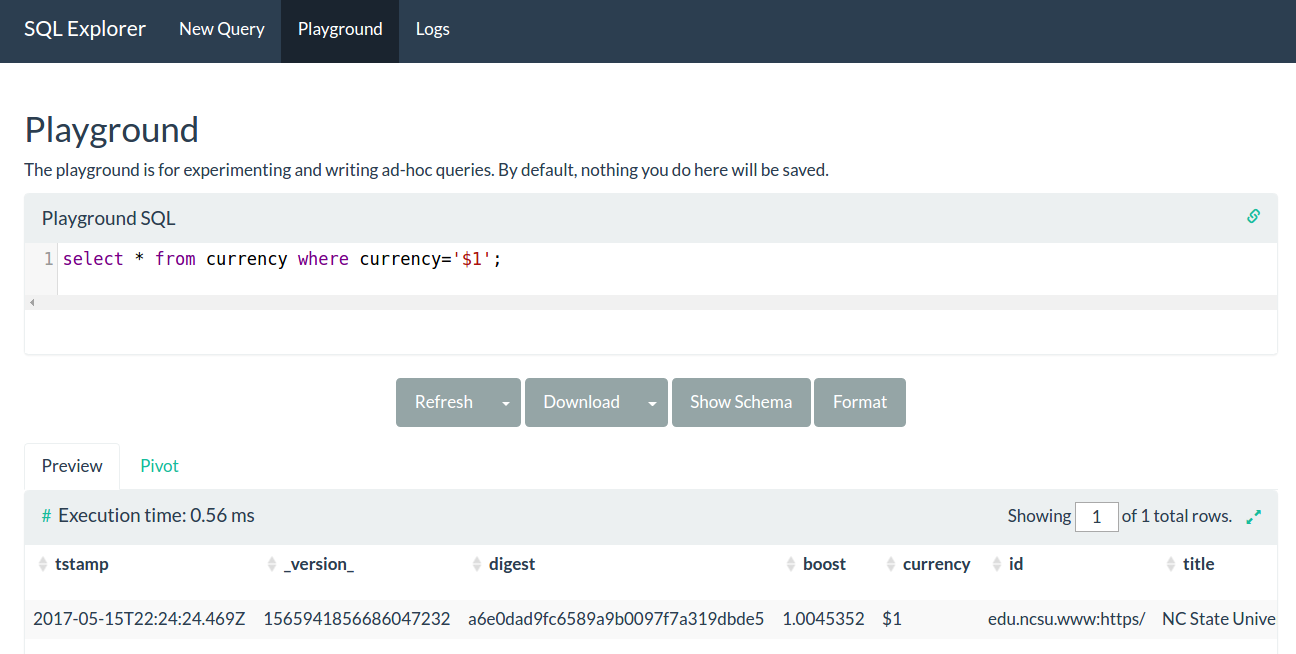
\includegraphics[width=16cm,height=7cm]{screenshots/result-portrait.png}
  \caption{Data Visualization using Portrait}
  \label{result-portrait}
\end{figure}


\clearpage
